\section{Application Programming Interface}

\subsection{Matching Engine (org.sidiff.matching.api)}

\class{org.sidiff.matching.api}{MatchingFacade}{none}{
Die Klasse \textit{Matching Facade} stellt Methoden zur Verfügung, um Korrespondenzen zwischen mehreren Modellen zu berechnen und zu serialisieren.
}

\class{org.sidiff.matching.api.settings}{MatchingSettings}{BaseSettings}{
\begin{figure}[!h]
\centering
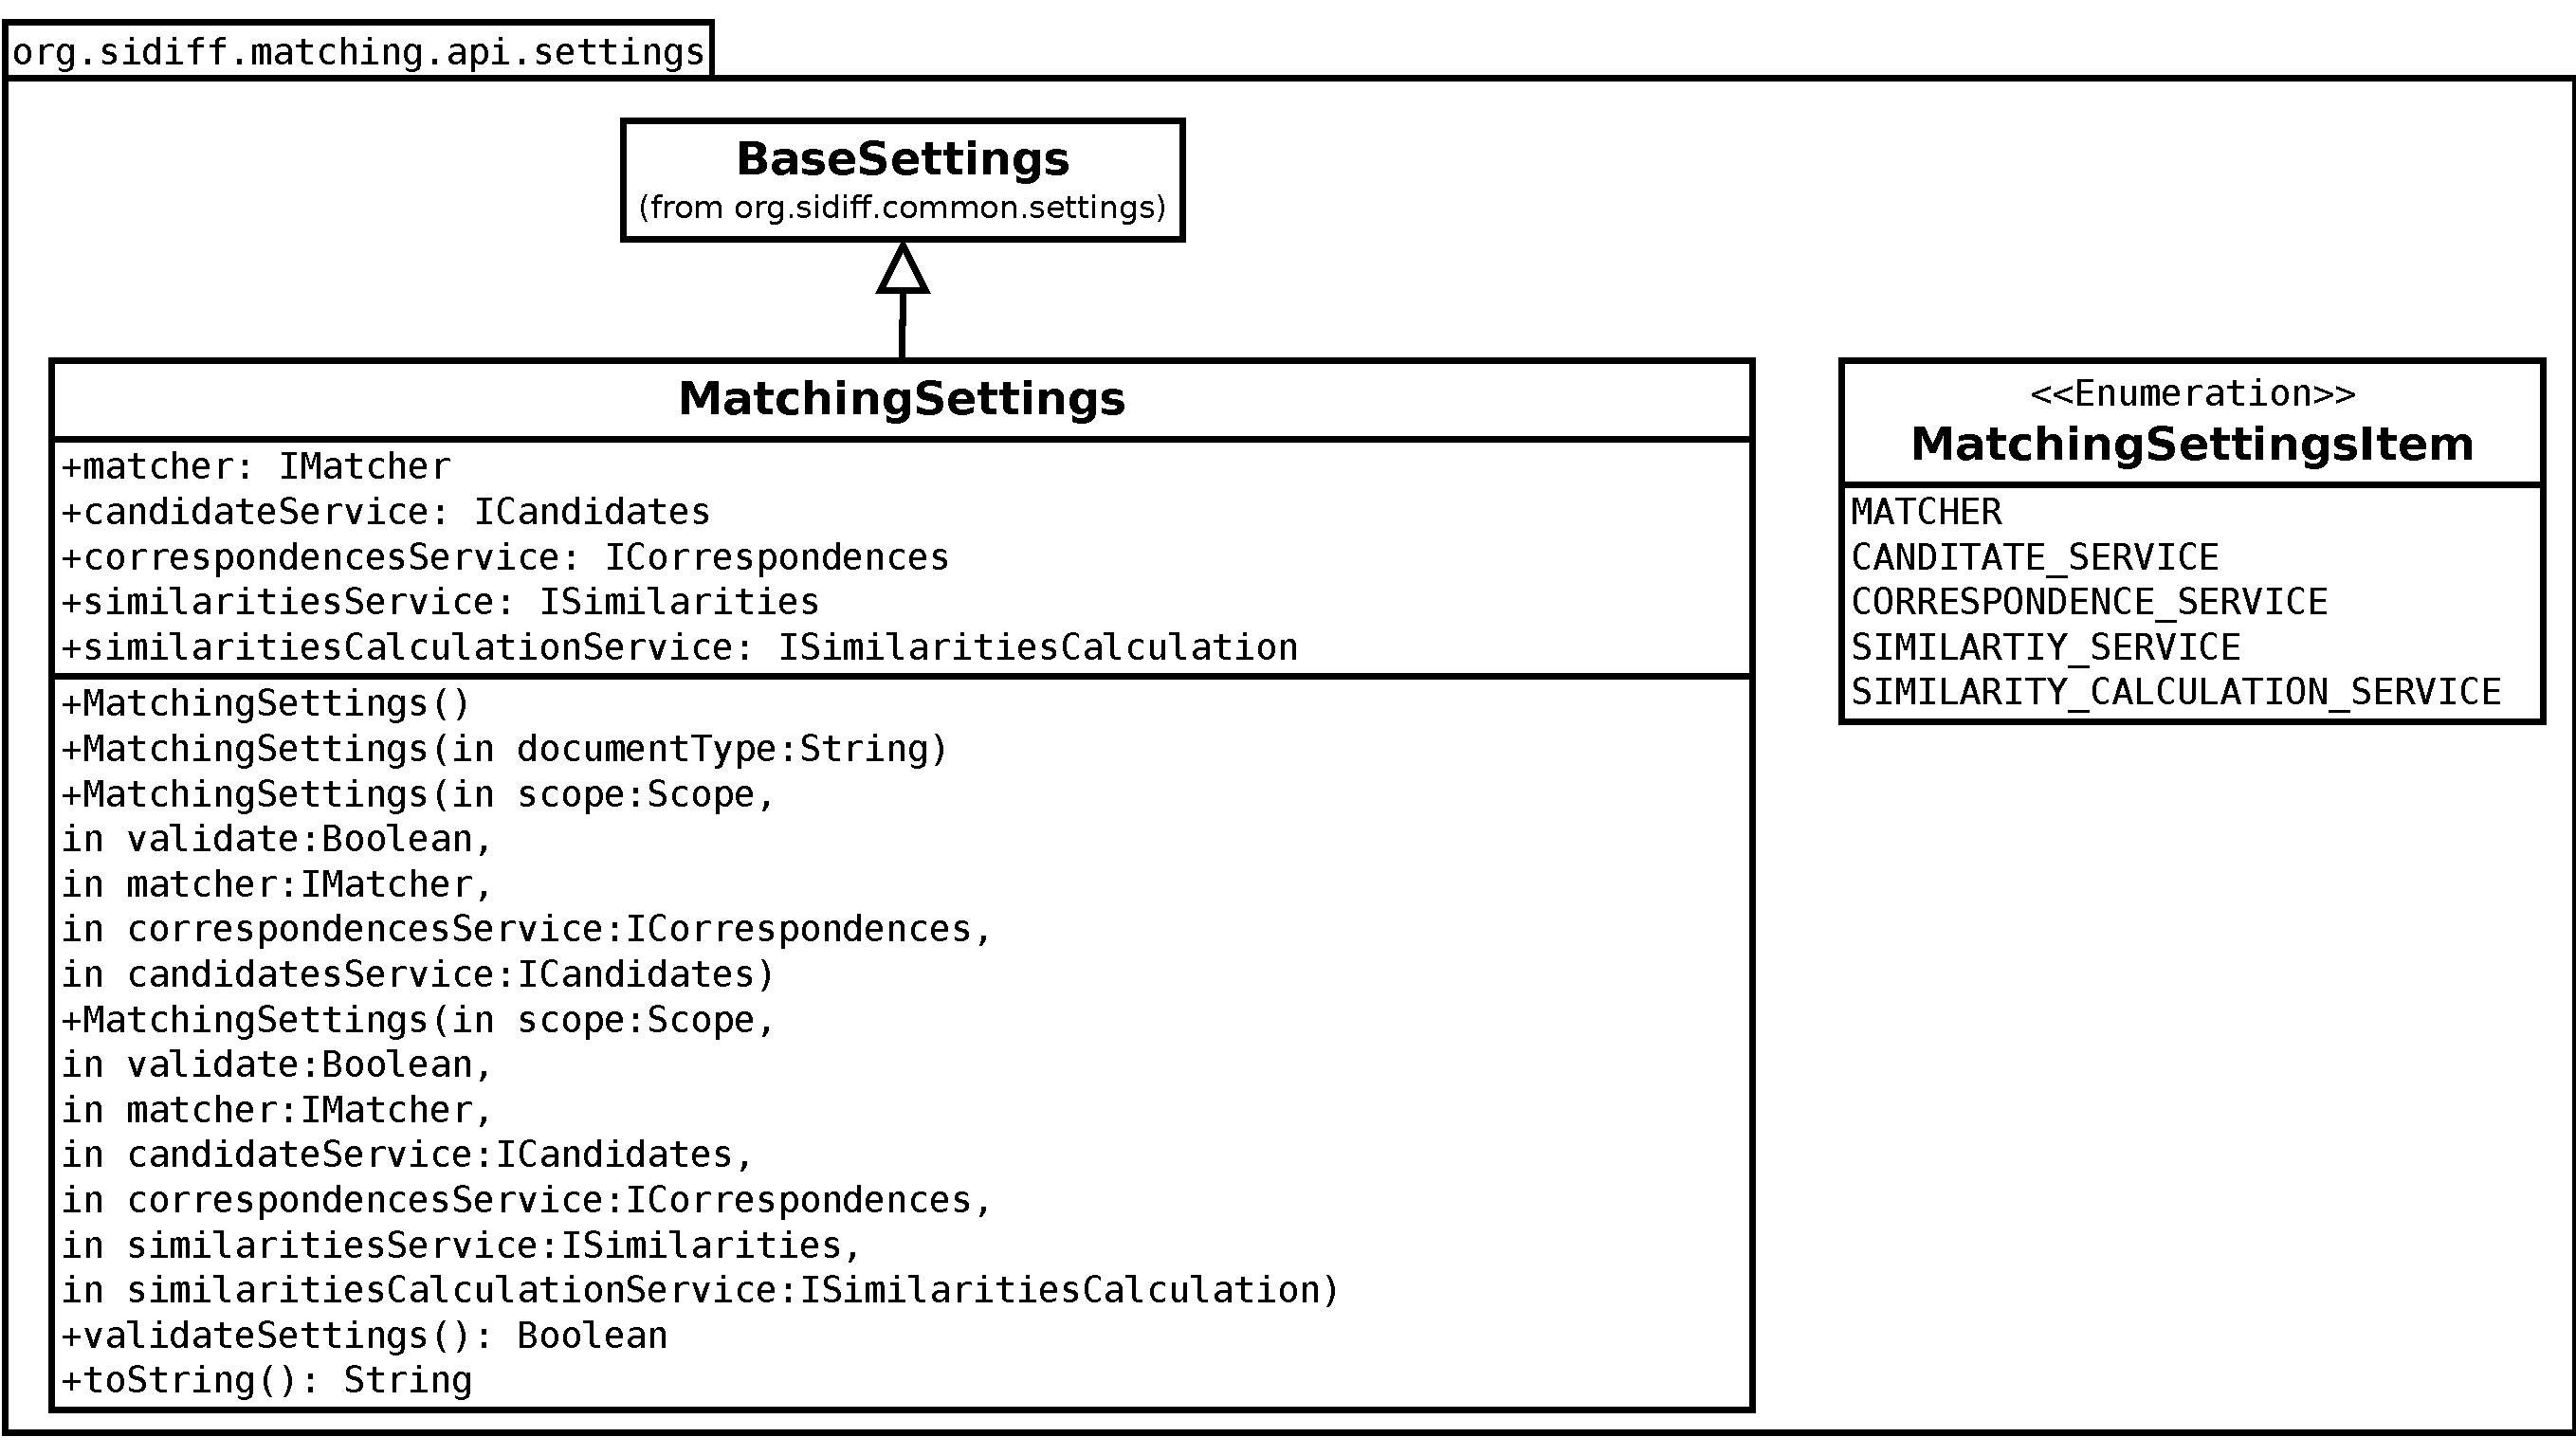
\includegraphics[width=0.75\textwidth]{images/api/settings_matching.pdf}
\caption{Matching Settings}
\label{fig:settings_matching}
\end{figure}
}

\subsection{Difference Derivator (org.sidiff.difference.technical.api)}

\class{org.sidiff.difference.technical.api}{TechnicalDifferenceFacade}{MatchingFacade}
{
Die Klasse \textit{TechnicalDifferenceFacade} stellt Methoden zur Verfügung, um eine technische Differenz zwischen zwei Modellen zu berechnen und zu serialisieren.\\
}

\class{org.sidiff.difference.technical.api.settings}{DifferenceSettings}{MatchingSettings}{
\begin{figure}[!h]
\centering
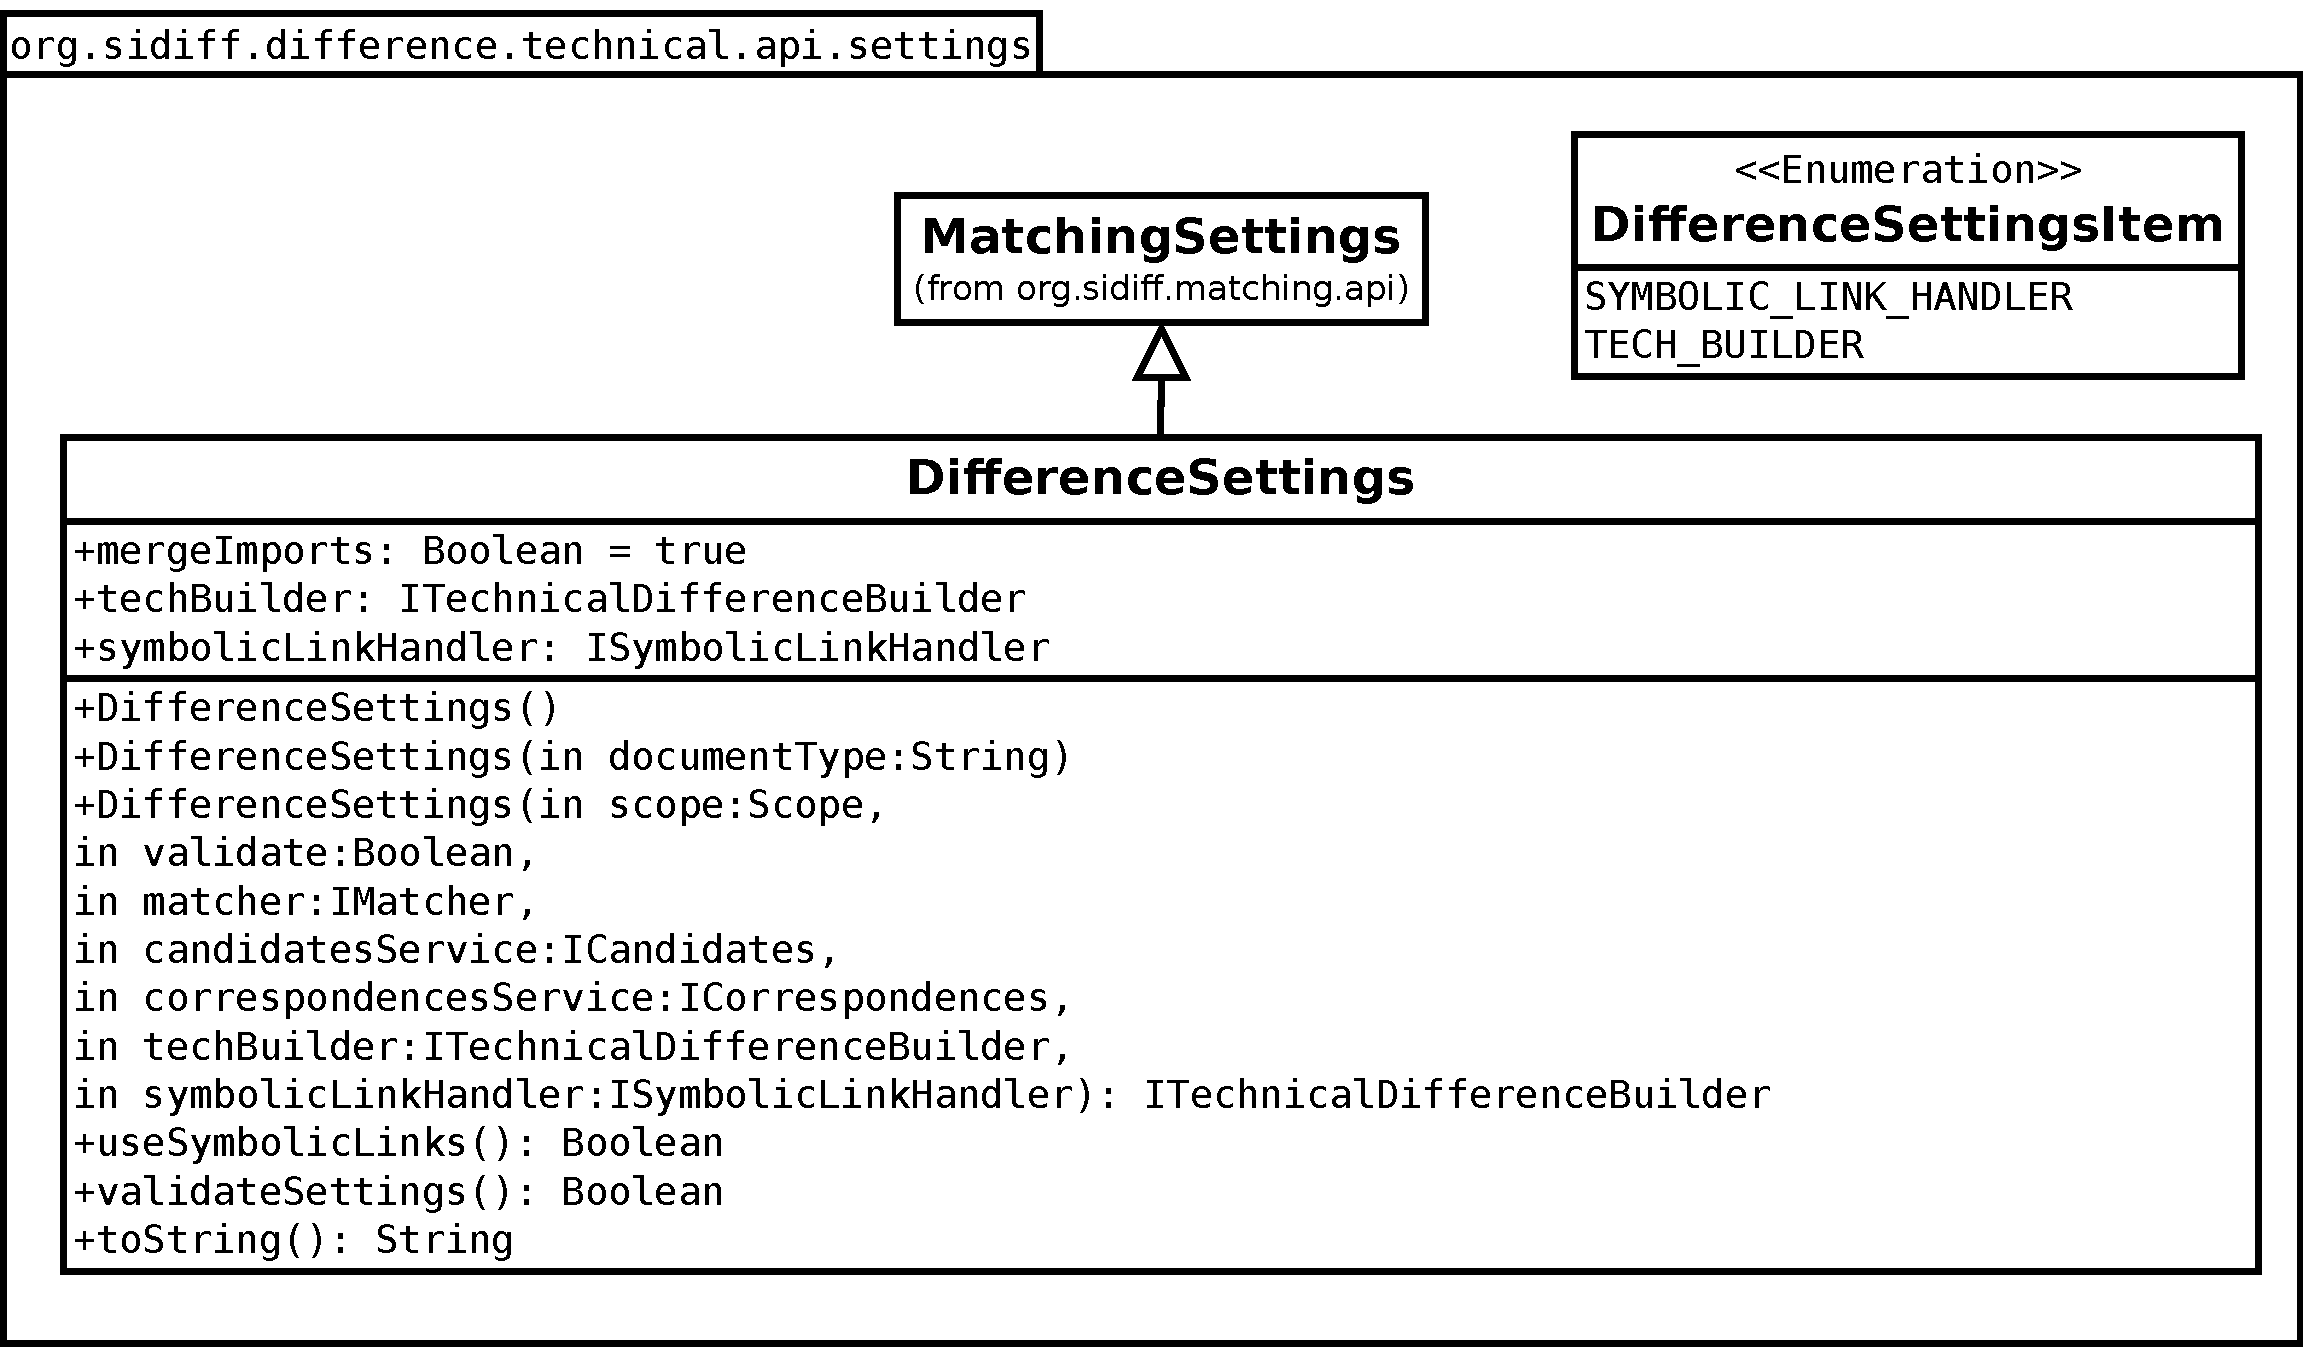
\includegraphics[width=0.75\textwidth]{images/api/settings_difference.pdf}
\caption{Difference Settings}
\label{fig:settings_difference}
\end{figure}
}

\subsection{LiftingEngine (org.sidiff.difference.lifting.api)}

\class{org.sidiff.difference.lifting.api}{LiftingFacade}{TechnicalDifferenceFacade}{
Die Klasse \textit{LiftingFacade} stellt Methoden zur Verfügung, um eine technische Differenz semantisch zu lfiten und zu serialisieren.}

\class{org.sidiff.difference.asymmetric.api}{AsymmetricDiffFacade}{LiftingFacade}{
Die Klasse \textit{AsymmetricDiffFacade} stellt Methoden zur Verfügung, um eine geliftete, ausführbare, asymmetrische Differenz zu berechnen und zu serialisieren.}

\class{org.sidiff.difference.lifting.api.settings}{LiftingSettings}{DifferenceSettings}{
\begin{figure}[!h]
\centering
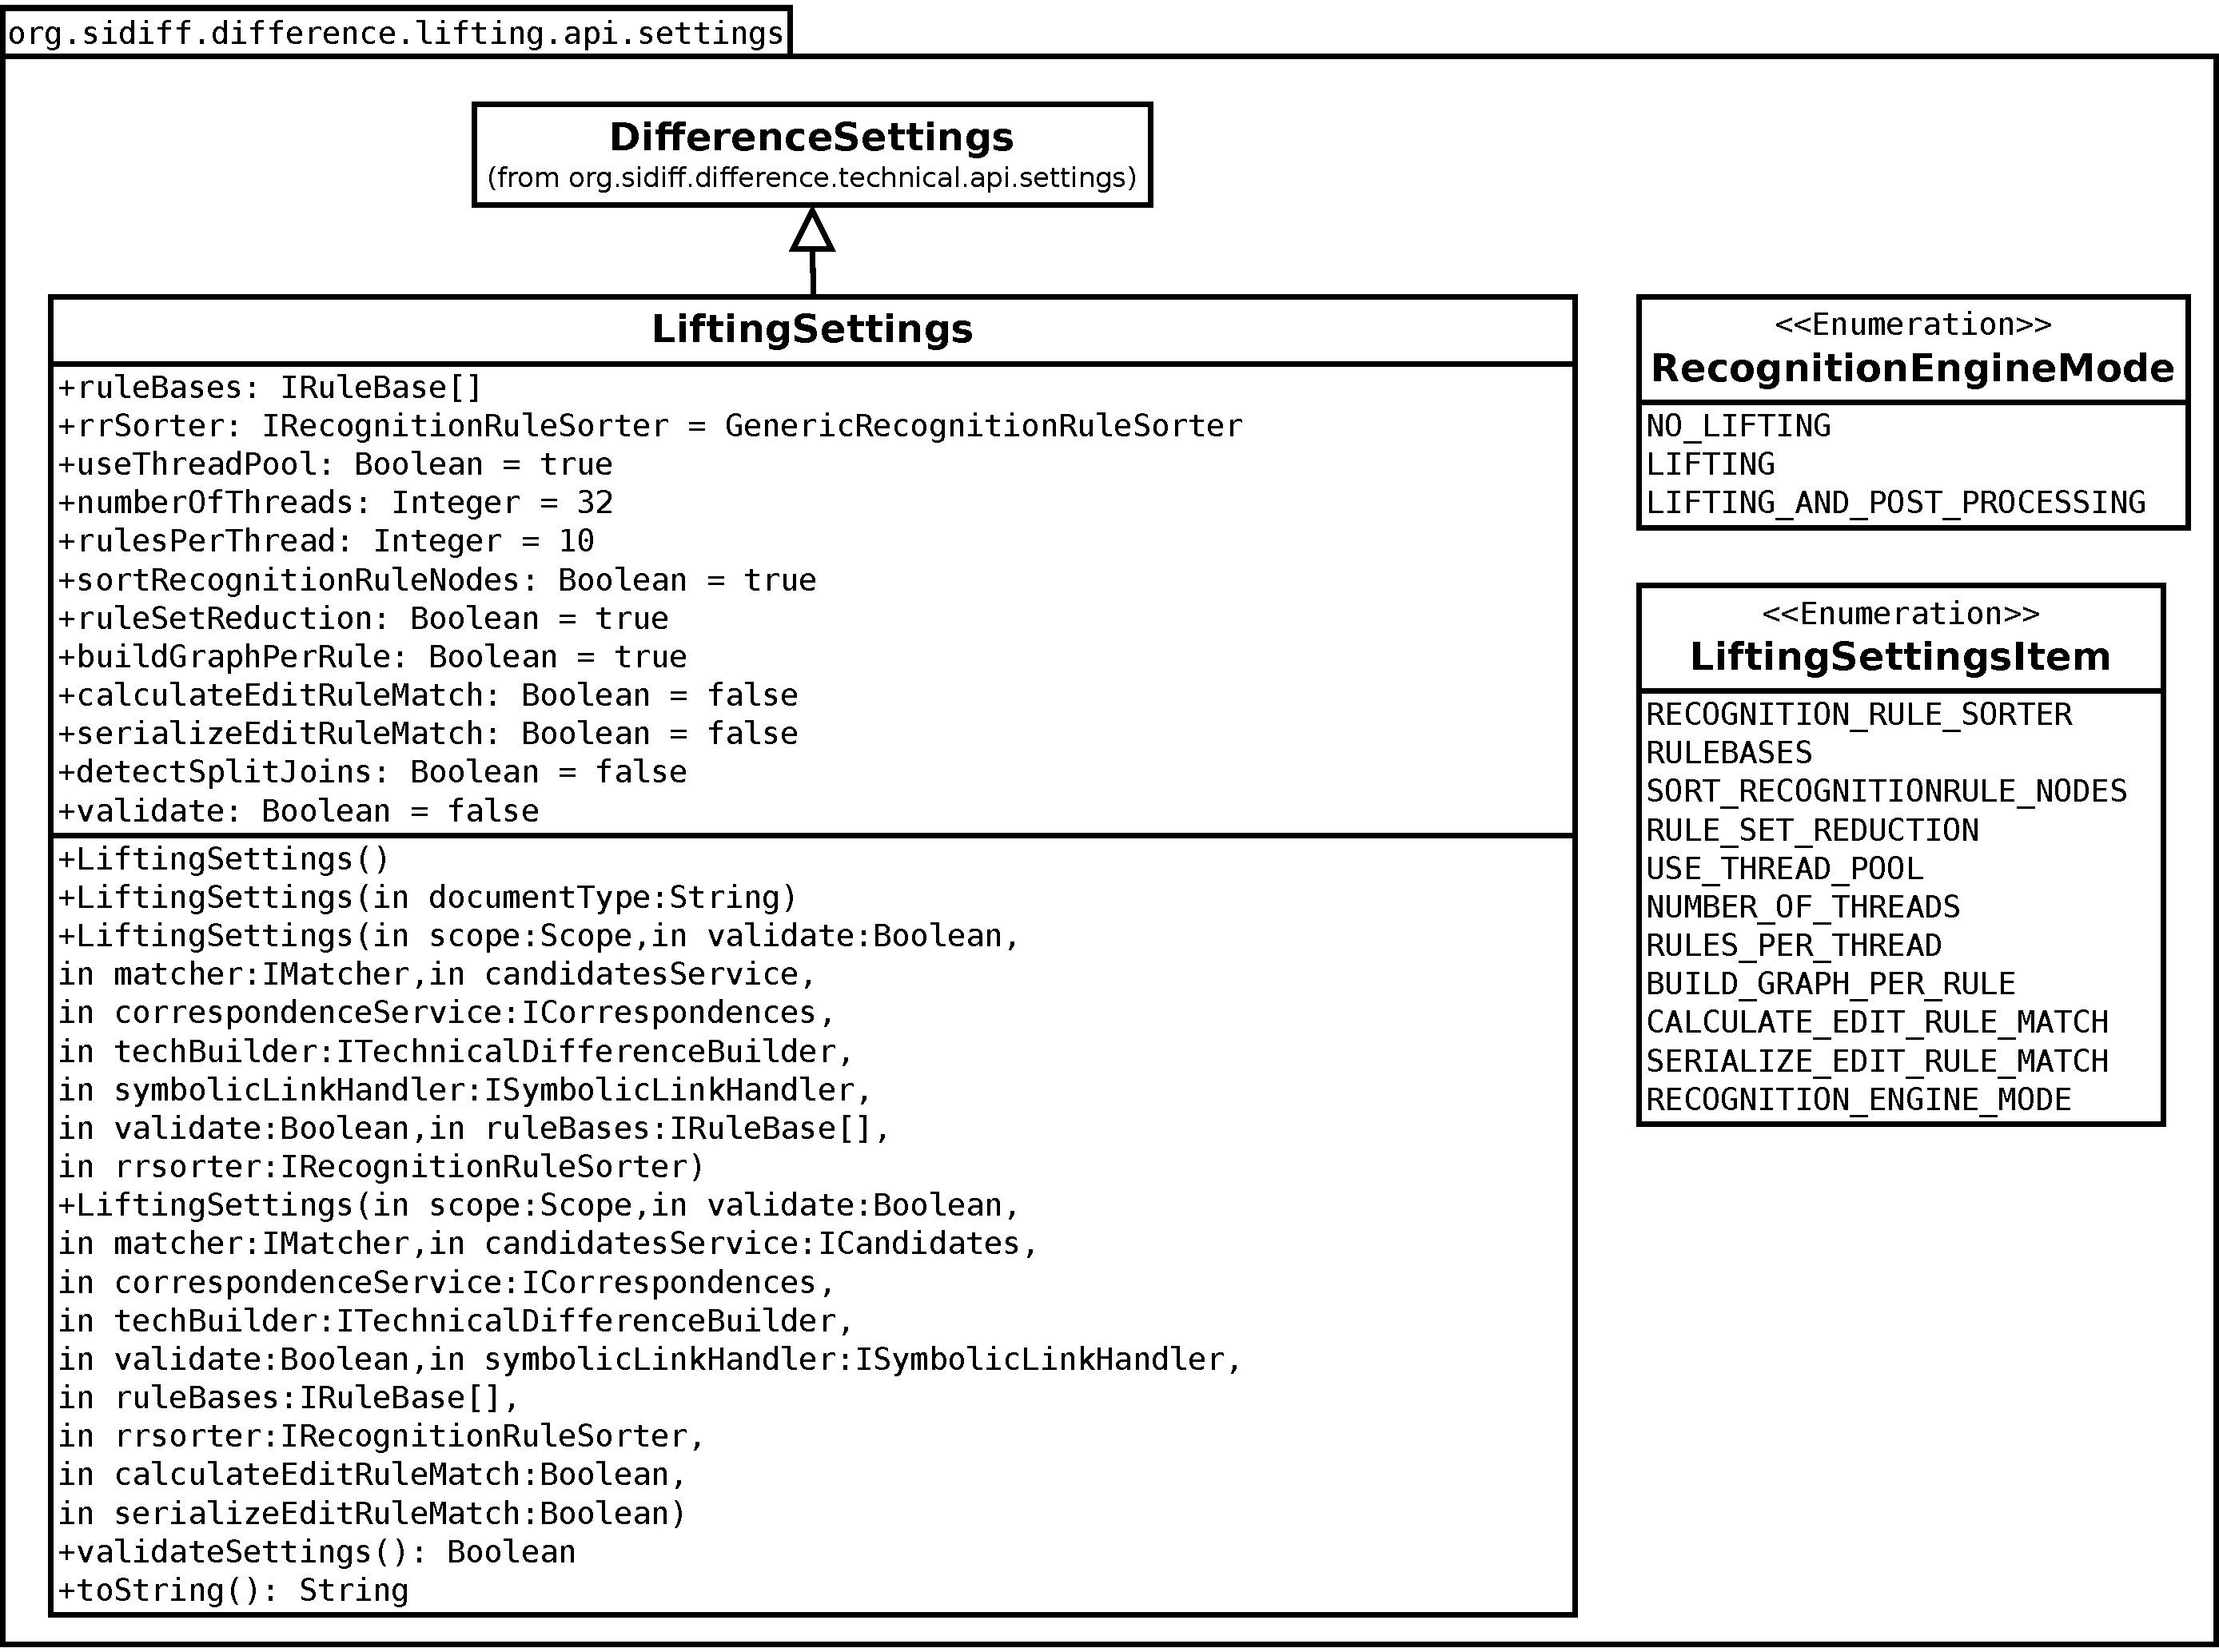
\includegraphics[width=0.75\textwidth]{images/api/settings_lifting.pdf}
\caption{Lifting Settings}
\label{fig:settings_lifting}
\end{figure}
}